% Tipo de documento y tamaño de letra
\documentclass[letterpaper,10pt,twoside,onecolumn]{article}

\textwidth=12cm
% Preparando para documento en Español.
% Para documento en Inglés no hay que hacer esto.
\usepackage[spanish]{babel}
\usepackage{graphicx}
\selectlanguage{spanish}
\usepackage[utf8]{inputenc}
\begin{document}
 
\title{REPORTE PRODUCTO 7}

\author{Ana Magdalena Sotomayor} 

\maketitle 
\section{INTRODUCCION}
Las mareas son los  ascensos y descensos periódicos de todas las aguas oceánicas, incluyendo las del mar abierto, los golfos y las bahías, la cual resulta de la atracción gravitatoria de la Luna y del Sol sobre el agua y la propia Tierra.
\subsection{Las mareas Lunares}
La Luna, al estar mucho más cerca de la Tierra que el Sol, es la causa principal de las mareas. Cuando la Luna está justo encima de un punto dado de la superficie de la Tierra, ejerce una fuerza de atracción del agua, que hace que se eleva sobre su nivel normal. La cresta de onda situada bajo la Luna se llama marea directa, y la del lado diametralmente opuesto de la Tierra se llama marea opuesta. En ambas crestas, prevalece la condición conocida como de marea alta, mientras que a lo largo de la circunferencia formada por las zonas perpendiculares al eje de mareas directa y opuesta se producen fases de marea baja.

Las mareas alta y baja se alternan en un ciclo continuo. En la mayoría de las costas del mundo se producen dos mareas altas y dos bajas cada día lunar, siendo la duración media de un día lunar 24 horas y casi un minuto. Una de las mareas altas está provocada por la cresta de marea directa y la otra por la cresta de marea opuesta.
\subsection{Las mareas solares}
El Sol provoca el ascenso de dos crestas de onda opuestas, pero como el Sol está lejos de la Tierra, su fuerza para crear mareas es un 46 por ciento menor que la Luna. El resultado de la suma de las fuerzas ejercidas por la Luna y el Sol es una onda compuesta por dos crestas, cuya posición depende de las posiciones relativas del Sol y de la Luna en un instante dado. Durante los periodos de Luna nueva y llena, cuando el Sol, la Luna y la Tierra están alineados, las ondas solar y lunar coinciden.

Cuando la atracción del Sol se suma a la de la Luna las mareas son grandes y las llamamos mareas vivas. Las alturas de las mareas vivas están regidas por la distancia de la Luna a la Tierra, siendo más grandes en el Perigeo, es decir, cuando la Luna está más cerca de la Tierra, y más pequeñas en el Apogeo, es decir, cuando la Luna se encuentra mas lejos de la Tierra .
\subsection{Esquema de las mareas}
\subsection{Tipos de Mareas}
 Mareas semidiurnas, cuando hay dos pleamares y dos bajamares en cada día lunar,con las dos pleamares alcanzando niveles del agua muy parecidos.

 Mareas diurnas, solamente una pleamar y una bajamar tienen lugar durante un
día lunar. Este tipo de mareas, baste más raras que las semidiurnas, se dan en la costa
norte del Golfo de Méjico, en el Mar de Java, en el Golfo de Tonkin y en algunos otros
lugares

Mareas mixtas. En este caso la altura de la marea presenta características comunes
a ambos tipos, diurna y semidiurna, simultáneamente, dando lugar a apreciables
diferencias entre los niveles del agua correspondientes a dos pleamares consecutivas.
En este tipo de mareas hay normalmente dos pleamares y dos bajamares por día
lunar pero ocasionalmente la marea adquiera carácter diurno. Este tipo de mareas son
comunes a lo largo de la costa Pacífica de Estados Unidos,
\includegraphics[scale=.50]{EsquemaMareas.jpg}

\section{HISTORIA}
El fenómeno de las mareas es conocido desde la antigüedad. Parece ser que Piteas (siglo IV a. C.) fue el primero en señalar la relación entre la amplitud de la marea y las fases de la Luna, así como su periodicidad. Plinio el Viejo (23-79) en su Naturalis Historia describe correctamente el fenómeno y piensa que la marea está relacionada con la Luna y el Sol. Mucho más tarde, Bacon, Kepler y otros trataron de explicar ese fenómeno, admitiendo la atracción de la Luna y del Sol. Pero fue Isaac Newton en su obra Philosophiae Naturalis Principia Mathematica («Principios matemáticos de la Filosofía Natural», 1687) quien dio la explicación de las mareas aceptada actualmente. Más tarde, Pierre-Simon Laplace (1749-1827) y otros científicos ampliaron el estudio de las mareas desde un punto de vista dinámico.

Isaac Newton realizó varios estudios científicos del comportamiento de las mareas y calculó la altura de éstas según la fecha del mes, la estación del año y la latitud. Más tarde, Simon Laplace complementó los estudios de Newton. 

A continuación se realizó un código en Fortran para el análisis de datos tomados en El Sargento durante aproximadamente 5 meses. 
Se crearon dos matrices, una de días muestreados (159 días x 48 muestras diarias) y otra mensual (5 meses x 1344 muestreos). 
A partir de esas matrices se realizaron los cálculos para conocer mínimos y máximos tanto mensuales como por día, e incluso para obtener las variantes de las mareas en un mismo día.

\section{CÓDIGO}

\begin{verbatim}
!Programa para graficar los datos de mareas tomados durante un periodo de tiempo
!para representar el comportamiento de las mareas, segun la hora del dia,
!temperatura y presion atmosferica
!Código por Ana M. Sotomayor
!-------------------------------------------------------------------------------------------

Module Parametros
     Implicit None
    integer, parameter :: puntos = 7632 !total de puntos
    integer, parameter :: dias = 159 !dias completos muestreados
    integer, parameter :: inicio = 286 !DOY inicial
    integer, parameter :: datos = 48 !Datos por dia
    integer, parameter :: datxmes = 1344
    integer, parameter :: dxmes = 28 !dias por mes lunar
    integer, parameter :: meses = 5 !Meses completos muestreados
    integer, parameter :: completos = 6720 !dias que completan los 5 meses
    integer, parameter :: semana = 7 !dias de la semana

End Module Parametros

Program Producto7
    Use Parametros
    implicit none
    integer :: i, j, k
    real :: xMax, xMin, dian, PromMin, PromMax
    real, dimension (1:5) :: Minmes, Maxmes,diamax, diamin, periodomax, periodomin
    real, dimension (1:dias) :: Mindia, Maxdia,  horamin, horamax
    real, dimension (1:puntos) :: PresAtm, Temp, NivAgua, DOY
    real, dimension (1:semana) :: Minam,HoraMinam,Maxam, HoraMaxam, Maxpm, HoraMaxpm, Minpm, HoraMinpm
    real, dimension (:,:), Allocatable :: Array,Arraymes
ALLOCATE (Array(dias,datos))
ALLOCATE (Arraymes(meses,datxmes))

  do i = 1, puntos, 1
    open (1, file = "data.csv", status="old")
    Read (1,*) PresAtm(i), Temp(i), NivAgua(i), DOY(i)
    open (2, file = "HNA.dat")
    open (3, file = "PresionNivelAgua.dat")
    open (4, file = "TempNivelAgua.dat")
    write (2,*) DOY(i), NivAgua(i) 
    Write (3,*) DOY(i), Temp(i) 
    write (4,*) DOY(i), PresAtm(i)
  end do
    close (1)
    close (2)
    close (3)
    close (4)
!Asignamos valores a la primera matriz (por dia)
i=1
   Open (2, file ="HNA.dat", status = "old")
   do  j = 1, dias, 1
     do k = 1, datos, 1  
       Read (2,*) DOY(i), NivAgua(i)
       Array (j,k) = NivAgua(i)
       i=i+1
     end do
   end do
  close (2)
!write (*,*) array

!Asignamos valores a la segunda matriz(por mes)
i=1
 Open (2, file ="HNA.dat", status = "old") 
 Do j=1,meses,1
	Do k = 1,datxmes,1
          Read (2,*) DOY(i), NivAgua(i)
          Arraymes (j,k)=NivAgua(i)
          i = i+1
	End do
End do
close (2)
!Write (*,*) arraymes


!Datos Minimos por mes
open (6, file="MinimosMes.dat")
 do j = 1, meses, 1
 xMin=0
     do k= 1,datxmes, 1
        if (Arraymes(j,k) .lt.  xMin) then
        xMin=Arraymes(j,k)
        dian=(j-1)*dxmes+k/48
        end if
     Minmes(j)=xMin
     diamin(j)= dian+inicio
     end do
 Write (6,*) diamin(j), Minmes(j)
 end do
close (6)

!Datos Maximos por mes
 open (7, file="MaximosMes.dat")
 do j = 1, meses, 1
 xMax=-1
     do k= 1, datxmes, 1
        if (Arraymes(j,k) .gt.  xMax) then
        xMax=Arraymes(j,k)
        dian=(j-1)*dxmes+k/48
        end if
        Maxmes(j)=xMax
        Diamax(j)=dian+inicio
     end do
     Write (7,*) diamax(j), Maxmes(j)
 end do
Close (7)

!Datos Maximos por dia
 open (8, file="Maximos.dat")
 do j = 1, dias, 1
    xMax = -1
    do k= 1, datos, 1
       if (Array(j,k) .gt.  xMax) then
       xMax=Array(j,k)
       end if
       Maxdia(j)=xMax
       horamax(j) = (j+inicio-1)+(k/48)
    end do
    Write (8,*) horamax(j), Maxdia(j)
end do
Close (8)

!Datos Minimos por dia
open (9, file="Minimos.dat")
do j = 1, dias, 1
     xMin=0 
     do k= 1, datos, 1
        if (Array(j,k) .lt.  xMin) then
        xMin=Array(j,k)
        end if
        Mindia(j)=xMin
        horamin(j) = (j+inicio-1)+(k/48)
     end do
     Write (9,*) horamin(j), Mindia(j)
end do
Close (9)

!Obtenemos los Periodos entre máximos mensuales

Do j=2,meses,1
Periodomax(j)=diamax(j)-diamax(j-1)
end do

Do j=2,meses,1
Periodomin(j)=diamin(j)-diamin(j-1)
end do

!Periodos promedio
PromMax=sum(Periodomax)/4
PromMin=sum(Periodomin)/4
 
!Calculemos el minimo semidiurno
Open (10, file= "Minimosam.dat")

do j = 1, semana*3, 1
   xMin =0
   do k = 1, datos/2, 1
     if (Array(j,k) .lt. xMin) then
         xMin = Array(j,k) 
     end if      
       Minam(j)=xMin
       horaminam(j) = (j+inicio)
    end do
    Write (10,*) horaminam(j), Minam(j)
end do
close (10)

open (12, file= "Minimospm.dat")
do j = 1, semana*3, 1
xMin =0
   do k = 25, datos, 1
     if (Array(j,k) .lt. xMin) then
         xMin = Array(j,k) 
     end if      
     Minpm(j)=xMin
     horaminpm(j) = (j+inicio)
   end do
Write (12,*) horaminpm(j), Minpm(j)
end do
close (12)

Open (11, file="Maximosam.dat")
do j = 1, semana*3, 1
xMax =-1
   do k = 1, datos/2, 1
      if (Array(j,k) .gt. Xmax) then
      Xmax = Array(j,k)
      end if
    Maxam(j)=Xmax
    horamaxam(j) = (j+inicio)+(k/48)
   end do
Write (11,*) horamaxam(j), Maxam(j)
end do
Close (11)


open (13, file="Maximospm.dat")
do j = 1, semana*3, 1
xMax =-1
   do k = 25, datos, 1
      if (Array(j,k) .gt. Xmax) then
      Xmax = Array(j,k)
      end if
    Maxpm(j)=Xmax
    horamaxpm(j) = (j+inicio)+(k/48)
   end do
Write (13,*) horamaxpm(j), Maxpm(j)
end do
close (13)

open (14, file="Datos salida.dat")

!write (14 ,*) 'nivel de marea maxima por dia', Maxdia
!write (14 ,*) 'nivel de marea minima por dia', Mindia
write (14,*) "---------------------------------------"
write (14,*) 'nivel de marea minima por mes', MinMes
write (14 ,*) 'nivel de marea maxima por mes', MaxMes
write (14,*) "---------------------------------------"
write (14 ,*) 'Periodos entre maximos por mes', periodomax
write (14 ,*) 'Periodos entre minimos por mes', periodomin
write (14,*) "---------------------------------------"
write (14,*) "El periodo promedio de maximos es", PromMax
Write (14,*) "El periodo promedio de Minimos es", PromMin


End Program producto7

\end{verbatim}
\pagebreak

\section{SALIDAS}
\subsection{Resultados Obtenidos}
Se formatearon los resultados en una tabla, obteniendo los siguientes datos:\\
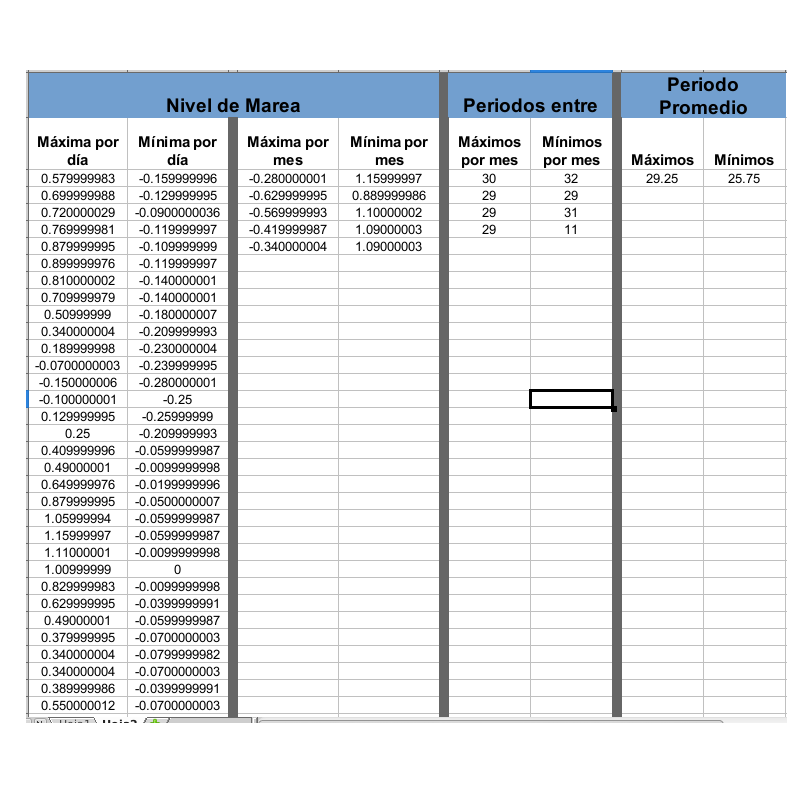
\includegraphics[scale=.50]{SalidaFormato.png}\\
Los datos se encuentran en el archivo Salida.xlsx
\pagebreak
\section{GRAFICAS}
Se obtuvieron las siguientes gráficas de los máximos y mínimos absolutos diarios\\
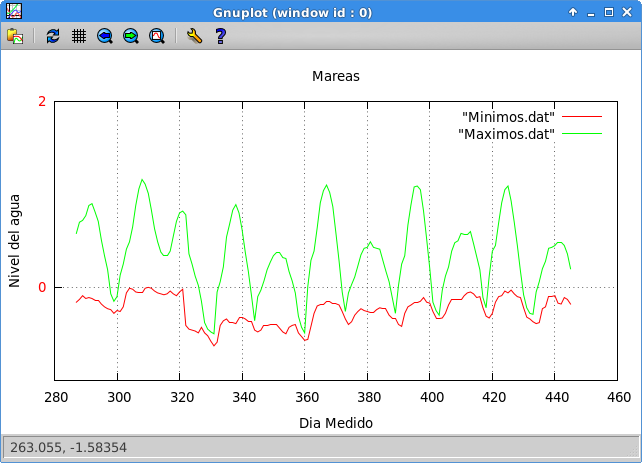
\includegraphics[scale=.50]{MinimosyMaximos.png}
GRAFICA\\
Y los siguientes datos que representan los máximos y mínimos mensuales durante el período muestreado\\
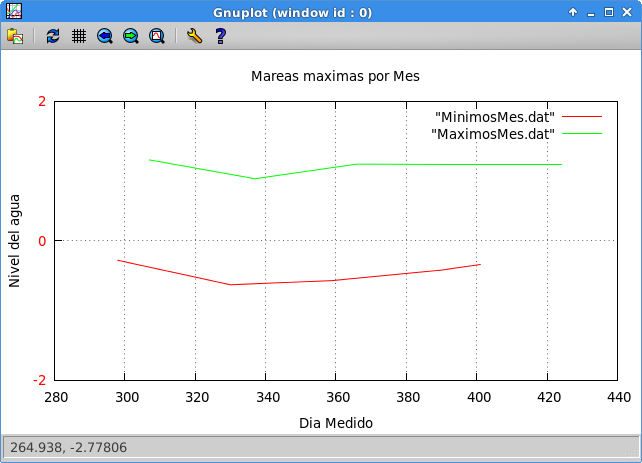
\includegraphics[scale=.55]{MaxyMinMes.png}
Por último se realizaron las graficas para conocer el tipo de mareas resultantes
obteniendo los siguientes resultados:
\includegraphics[scale=.50]{Mindiurnos.png}
GRAFICA\\
\includegraphics[scale=.55]{Maxdiurnos.png}\\
con lo anterior podemos observar que durante el día se tienen dos mareas máximas y dos mínimas con valores parecidos, por lo que podemos concluir que las mareas del Estero El Sargento, son mareas semidiurnas.

% Nunca debe faltar esta ultima linea.
\end{document}